
\chapter{IMPLEMENTATION}

\section{Reference Implementation}

Alongside this publication, we provide a reference implementation of OnioNS. We utilize C++11, the Botan cryptographic library, the Standard Template Library's (STL) implementation of Mersenne Twister, and the libjsoncpp-dev library for JSON encoding. We develop in Linux Mint and compile for Ubuntu Vivid, Utopic, Trusty, and their derivatives. Our software is built on Canonical's Launchpad online build system and is available online at \url{https://github.com/Jesse-V/OnioNS}. 

\section{Prototype Design}

We have developed an OnioNS prototype that implements the Domain Query protocol. In this initial prototype, we use a static server, a single fixed Create Record, and a hidden service that we deployed at onions55e7yam27n.onion. Although our implementation is primarily a seperate software package, we made necessary modifications to the Tor client software to intercept the .tor pseudo-TLD, pass the domain to the OnioNS client over inter-process communication (IPC), and receive and lookup the returned hidden service address. We diagram the relationships between our prototype's components in Figure \ref{fig:prototypeDiagram}.

Our prototype's works as follows:

\begin{enumerate}
	\item The user enters in ``example.tor'' into the Tor Browser.
	\item The Tor Browser sends ``example.tor'' to Tor's SOCKS port for resolution.
	\item The Tor client intercepts ``*.tor'', places the lookup in a wait state, and sends ``example.tor'' to the OnioNS client over a named pipe.
	\item The OnioNS client communicates with Tor's SOCKS port and negotiates a connection to the static OnioNS server.
	\item The OnioNS client performs a level 0 Domain Query to the server.
	\item The server responds with the Create Record containing ``example.tor''.
	\item The client writes ``onions55e7yam27n.onion'' to the Tor client over another named pipe.
	\item The Tor client resumes the lookup and overrides the original ``example.tor'' lookup with ``onions55e7yam27n.onion''.
	\item The Tor client contacts the OnioNS hidden service and passes the webpage to the Tor Browser.
	\item The Tor Browser displays the website contents and preserves the ``example.tor'' domain name.
\end{enumerate}

\begin{figure}[htbp]
	\centering
	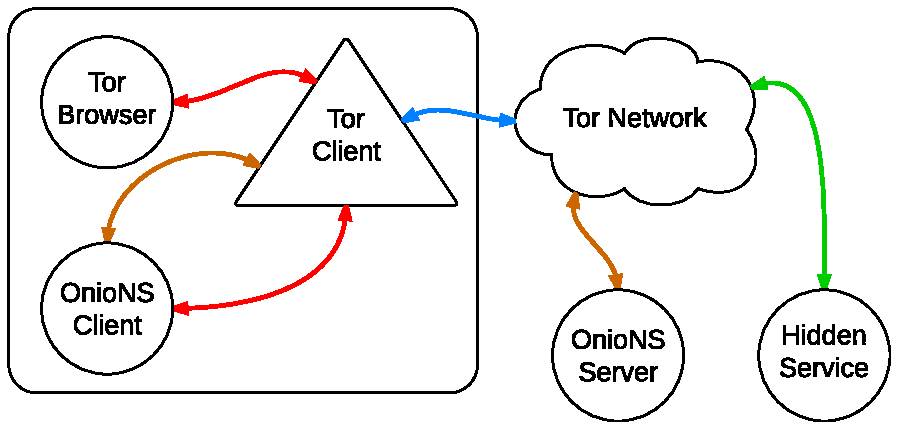
\includegraphics[width=0.75\textwidth]{images/LucidCharts/OnioNS_Prototype.pdf}
	\caption{Our OnioNS prototype involves five components: the Tor Browser, a modified Tor client, a OnioNS client, a OnioNS server, and the destination hidden service. The Tor Browser passes an unknown .tor domain to the OnioNS through the Tor software (shown in red) which resolves the domain anonymously over a Tor circuit (orange) to remote resolver. Finally, the Tor software contacts the destination server via the normal hidden service protocol (green). The Tor Browser communicates to the Tor client over its SOCKS port, while the OnioNS client communicates over named pipes (red) and Tor's SOCKS port (orange).}
	\label{fig:prototypeDiagram}
\end{figure}

\subsection{Challenges}

We encountered two significant challenges while implementing the prototype. 

Our first modification to the Tor software used blocking I/O for communication with the OnioNS client. This caused Tor's event loop to pause while the OnioNS was resolving the domain name. When the OnioNS client attempted to use Tor to construct a circuit to the OnioNS server, Tor could not respond as it was waiting on I/O. This resulted in an unresolvable deadlock. After collaboration with several Tor developers we migrated our Tor modification to libevent, a software library that enables asynchronous event. Libevent is heavily used throughout Tor, Google Chrome, ntpd, and other software. Libevent enabled the OnioNS client to communicate over Tor, communicate with the remote OnioNS resolver, and return the hidden service address to Tor. Libevent then fired a callback method to contact the hidden service.

Our second challenge was telling Tor to place the resolution of the domain on hold. Previously, Tor would attempt to interpret the .tor domain and fail the lookup almost instantaneously. To resolve this, we placed the resolution in a waiting state. Then when OnioNS resolved the domain, our Libevent callback resumed the lookup, passed in the initial state, and allowed the lookup to continue as if a hidden service address had been requested in the first place. This allowed the Tor Browser to view the destination hidden service under a .tor domain name.

\subsection{Future Work}

In future work we will port the OnioNS client to Windows and migrate the Tor-OnioNS IPC from Unix named pipes to TCP sockets. Although named pipes work reliably in Unix-like operating systems, they are not easily compatible in the Windows family of operating systems. Going forward, we will expand our implementation and collaborate with Tor developers to merge it into Tor's repositories.


%\section{Experimentation}
%
%
%\emph{Todo: I will carry out experiments in test deployments of the Tor network and see what the demand is. I anticipate it being relatively lightweight. The proof-of-work will almost certainly be the computational bottleneck.}
%
%\emph{Bandwidth, CPU, RAM, latency for clients to be determined...}

%demand on participating nodes to be determined...

%Unlike Namecoin, OnionNS' \emph{page}-chain is of $ L $ days in maximal length. This serves two purposes:

%\begin{enumerate}
%	\item Causes domain names to expire, which reduced the threat of name squatting.
%	\item Prevents the data structure from growing to an unmanageable size.
%\end{enumerate}

%\subsection{Proof-of-work}
%
%\emph{What are the optimal parameters for scrypt? What are the implications of setting it too high or too low?}
%
%\emph{How much bandwidth and time does this take?}
%
%\emph{How does the bandwidth and CPU load scale in response to a larger Quorum? Assuming reasonable clockskew, how off will the exchanges be? Are there any race conditions that need to be resolved?}
%
%\emph{Queres: How long does this take, and how can we improve efficiency? Can clients on even low-end hardware calculate the proof-of-work?}
%
%
%\section{Results}
%
%
%\emph{This will be expanded/rewritten once I finish implementation and deploy it in test/prototyping networks. I plan on using Chutney.}
